\chapter{\uppercase{PROSPECT Analysis Framework and Calibration}}

Events in the PROSPECT detector begin as bursts of scintillation in the liquid scintillator. 
In order to transform these events of light into physics data several steps have to be taken, including position reconstruction and energy calibration. 
This chapter will outline how these processes are performed, but before that is done a key component of the PROSPECT analysis, pulse shape discrimination, must be presented.

\section{Pulse Shape Discrimination}

Physics events in the PROSPECT detector, such as neutron captures on $^6$Li, produce scintillation light through ionization that is transported by way of the reflecting panels to individual PMTs. 
As described in Section~\ref{sec:DAQ}, these signals are processed by CAEN waveform digitizers and are only accepted if they pass the segment and ZLE thresholds.
Due to the nature of the liquid scintillator the shape of the digitized waveforms is defined by the ionization density of a given event.
Lower ionization density events, such as electrons, have a faster scintillator decay time causing less light in the ``tail" of the waveform compared to higher density events like proton recoils, as seen in Figure~\ref{fig:psddefine}. 

This allows the definition of a pulse shape discrimination (PSD) factor as the ratio of the signal in the tail versus the total waveform,
\begin{equation}
	PSD =  \frac{\int_{tail:start}^{tail:end}Qdt}{\int_{-\infty}^{\infty}Qdt}
\end{equation}
The tail area of a given waveform is defined as the window 44 - 100 ns after the time of the half-height leading edge. 
The total area is defined as the window -12 - 100 ns relative to the same leading edge time. 
An example of these windows on a typical pulse can be seen in Figure~\ref{fig:psddefine}.
Use of the PSD parameter, along with energy, provides clear separation between neutron captures on $^6$Li and other event classes such as electron recoils. 
An example of this for a single segment can be seen in Figure~\ref{fig:psdvss}, where a pseudo-energy is calculated using the integrated pulse area of each PMT, S$_0$ and S$_1$.

\begin{figure}[t]
	\centering
	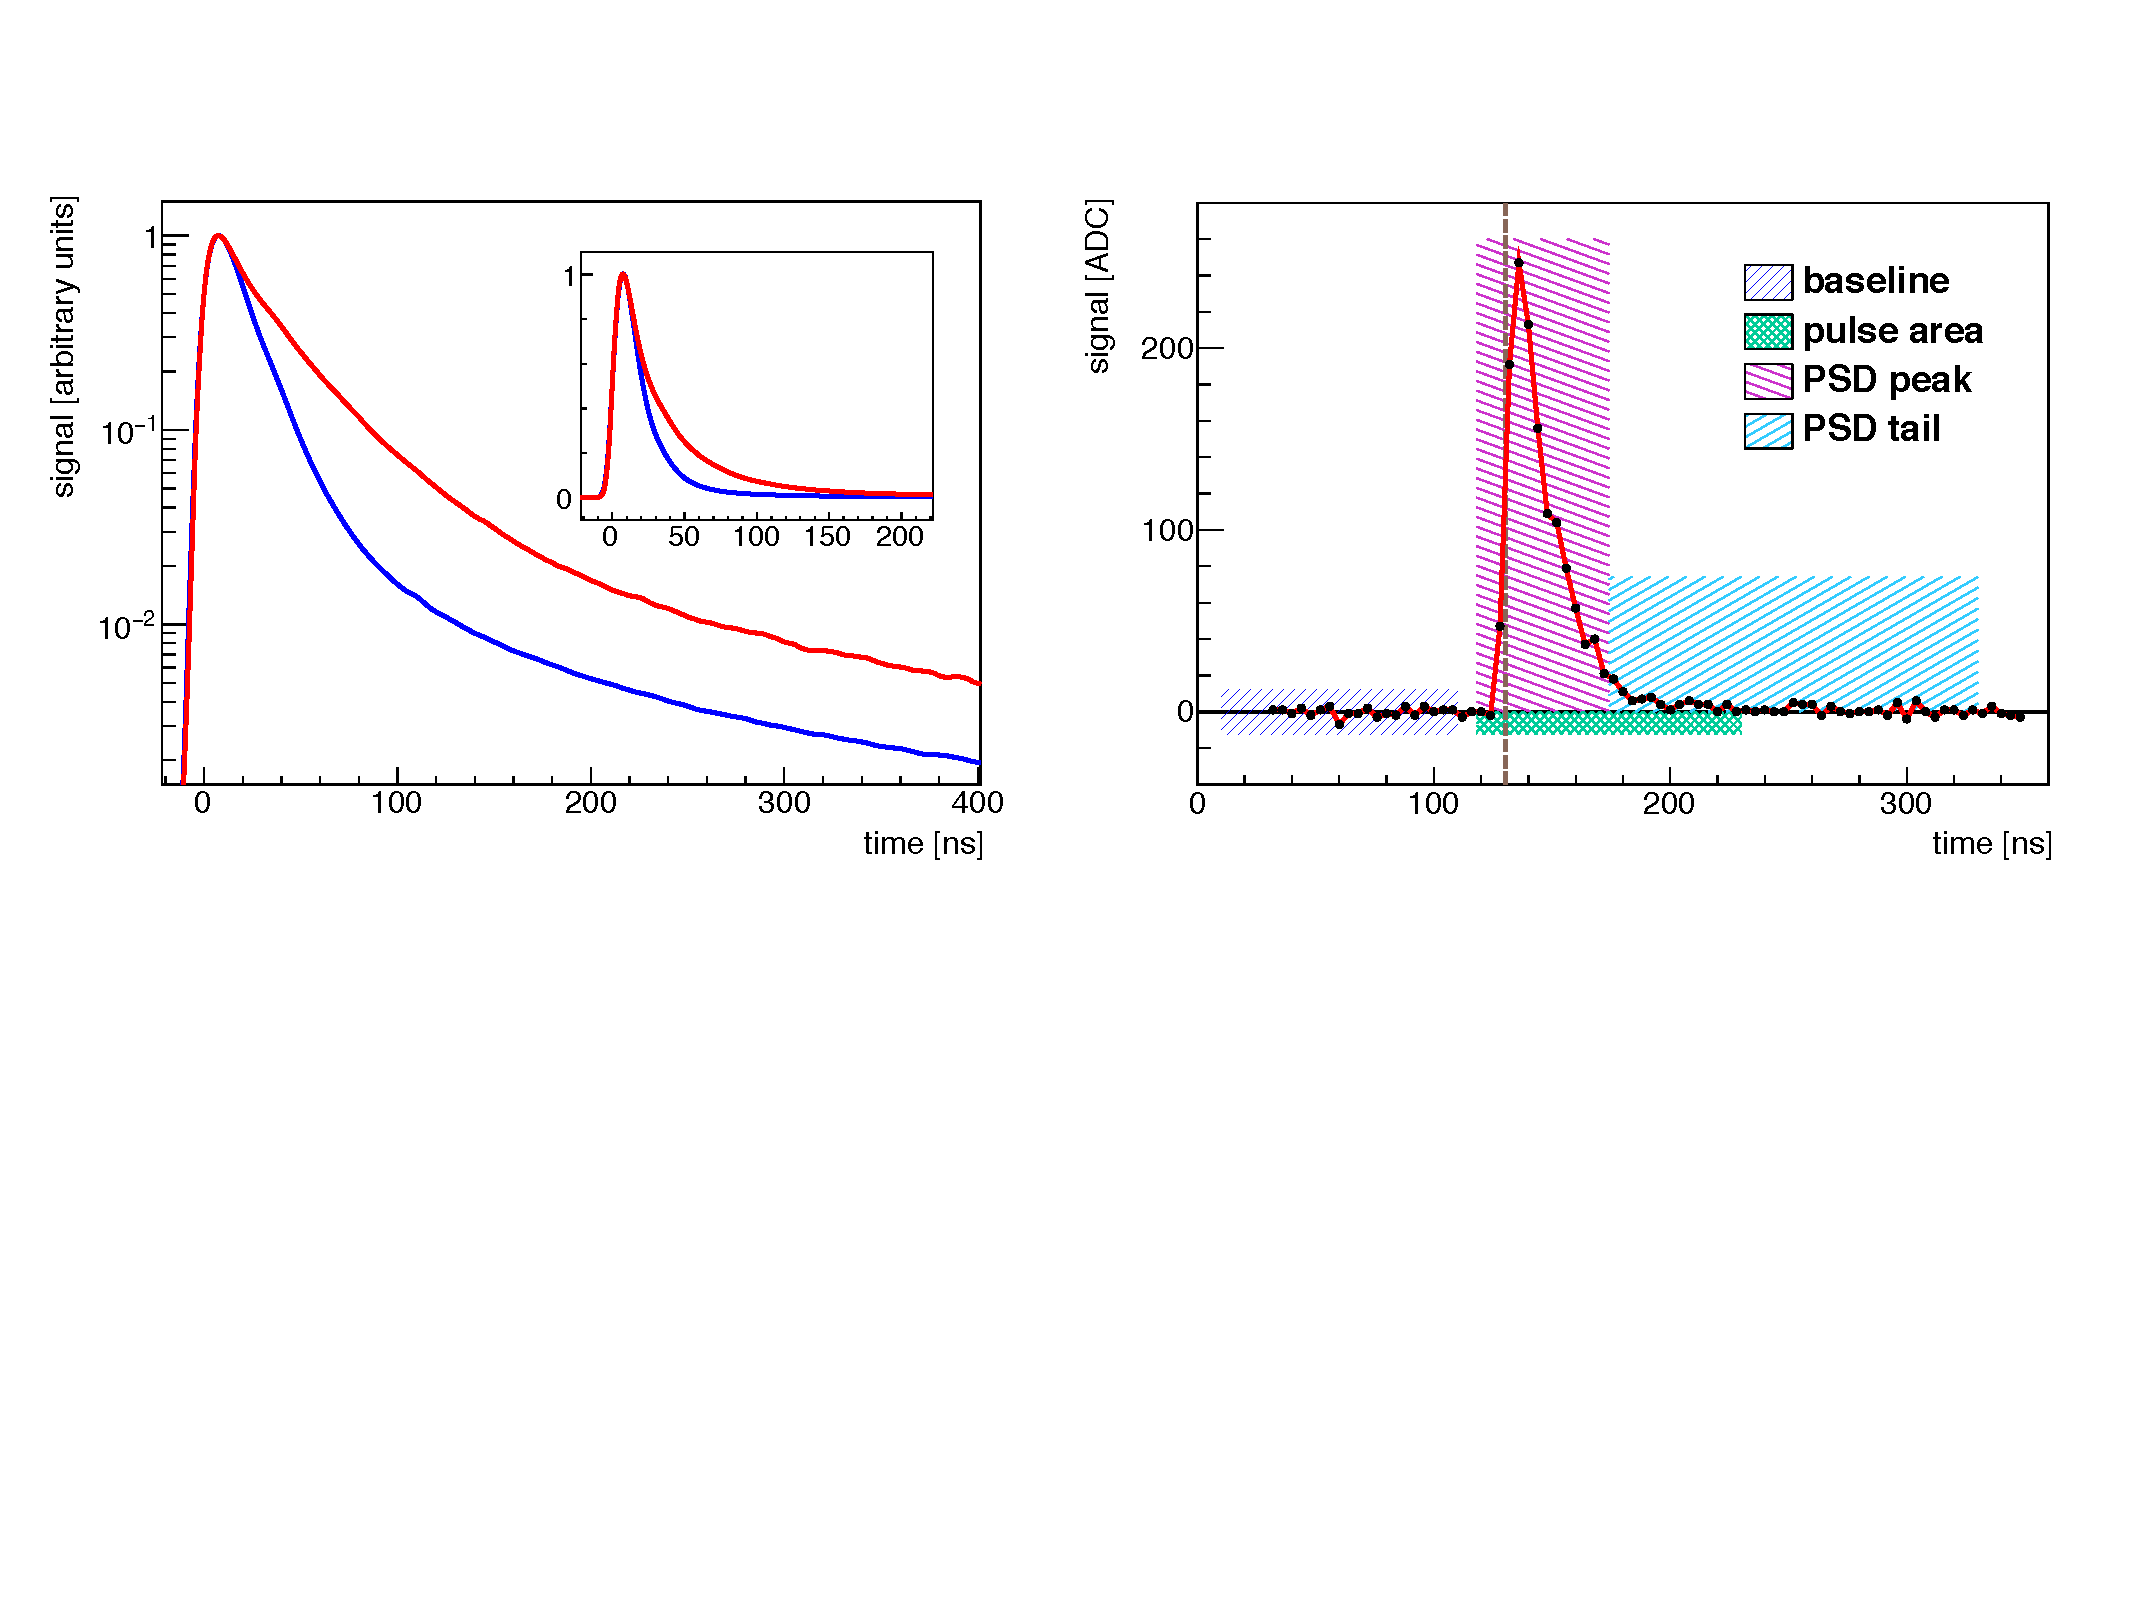
\includegraphics[width=0.99\linewidth]{tex/5-analysis-images/PSD_Define}
	\caption[Typical waveform]{(Left) Averaged waveforms from electrons (lower, blue) and proton recoils (upper, red) \cite{MM:2773}. The inset panel shows the same waveforms on a linear y axis. (Right) Example analysis of a typical pulse \cite{MM:2764}. The half-height leading edge timing (dashed vertical) determines windows for baseline subtraction, pulse area, and PSD. }
	\label{fig:psddefine}
\end{figure}

\begin{figure}[h]
	\centering
	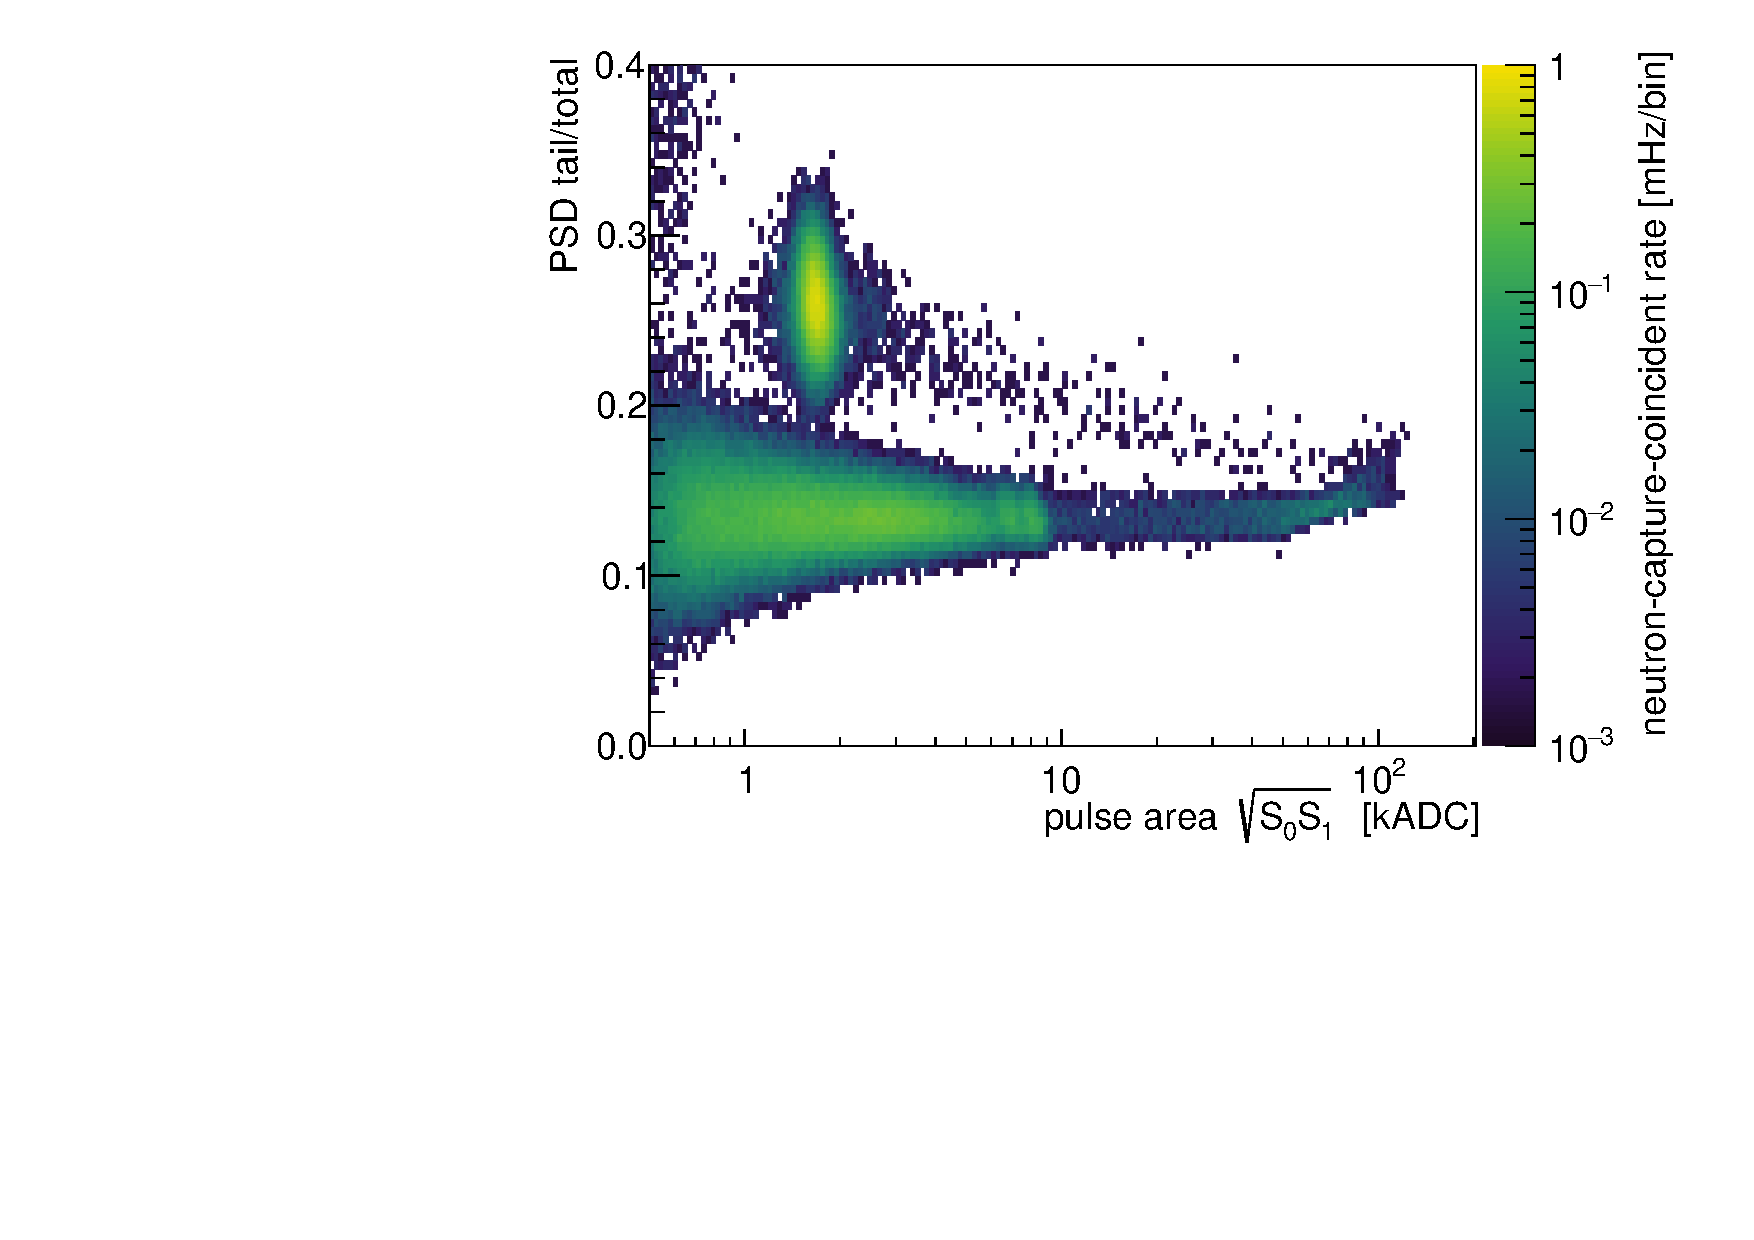
\includegraphics[width=0.6\linewidth]{tex/5-analysis-images/PSD_vs_S}
	\caption[PSD vs. psuedo-energy for neutron coincident events]{PSD vs. pseudo-energy for neutron capture coincident events in a single segment \cite{MM:2731}. The neutron captures, outlined by the magenta rectangle, are clearly separated in PSD from electron-like events in the lower band.}
	\label{fig:psdvss}
\end{figure}


\section{Data Processing and Calibration}

For simplicity consider one event contained in one segment. 
Both PMTs in the segment will collect photons from this event that are saved as individual waveforms. 
These are analyzed and information such as pulse area and height in analog-to-digital converter (ADC) units, PSD, and arrival time are saved. 
The next step involves combining information from both PMTs, calibrating the energy, and reconstructing the position. 

%The PSD is calculated as an average of the individual PMTs PSD weighted by the number of photoelectrons, $N$,
%\begin{equation}
%	PSD = \frac{N_0PSD_0 + N_1PSD_1}{N_0 + N_1}
%\end{equation}

\subsection{Timing to Position Curves}

Through-going muons provide a large and consistent data set which can be used to reconstruct positions based on timing.
As muons travel through the pinwheel rod tabs the light transport is distorted in timing and magnitude. 
This creates a striping effect in the timing between the two PMTs, $dt$, versus the signal amplitude ($S_0 + S_1$) distribution as shown in Figure~\ref{fig:dtshobbes}.

The striping becomes even clearer when plotting $dt$ for events with signal amplitudes in the range  1$e$4 -  2$e$4 ADC for a single segment as shown in Figure~\ref{fig:hobbesfit}.
For each segment this distribution is first fit with an ``M"-shaped curve, $M(dt)$. 
Then, the residual structure is fit to a sinusoidal curve with a slowly varying phase shift term,
\begin{equation}
	n(dt) = M(dt)\left[1 + k\cos\left(\frac{2\pi}{\delta}\left(a~dt + b~dt^3\right)\right)\right]
\end{equation}
where $\delta$ = 78.5 mm is the average spacing between pinwheel tabs, and $k, a, b$ are fit parameters.
The inner phase term provides the position calibration $z(dt) = a~dt + b~dt^3$, whose resulting curves are shown in Figure~\ref{fig:zvsdt}.

\begin{figure}
	\begin{minipage}[t]{0.5\linewidth}
		\centering
		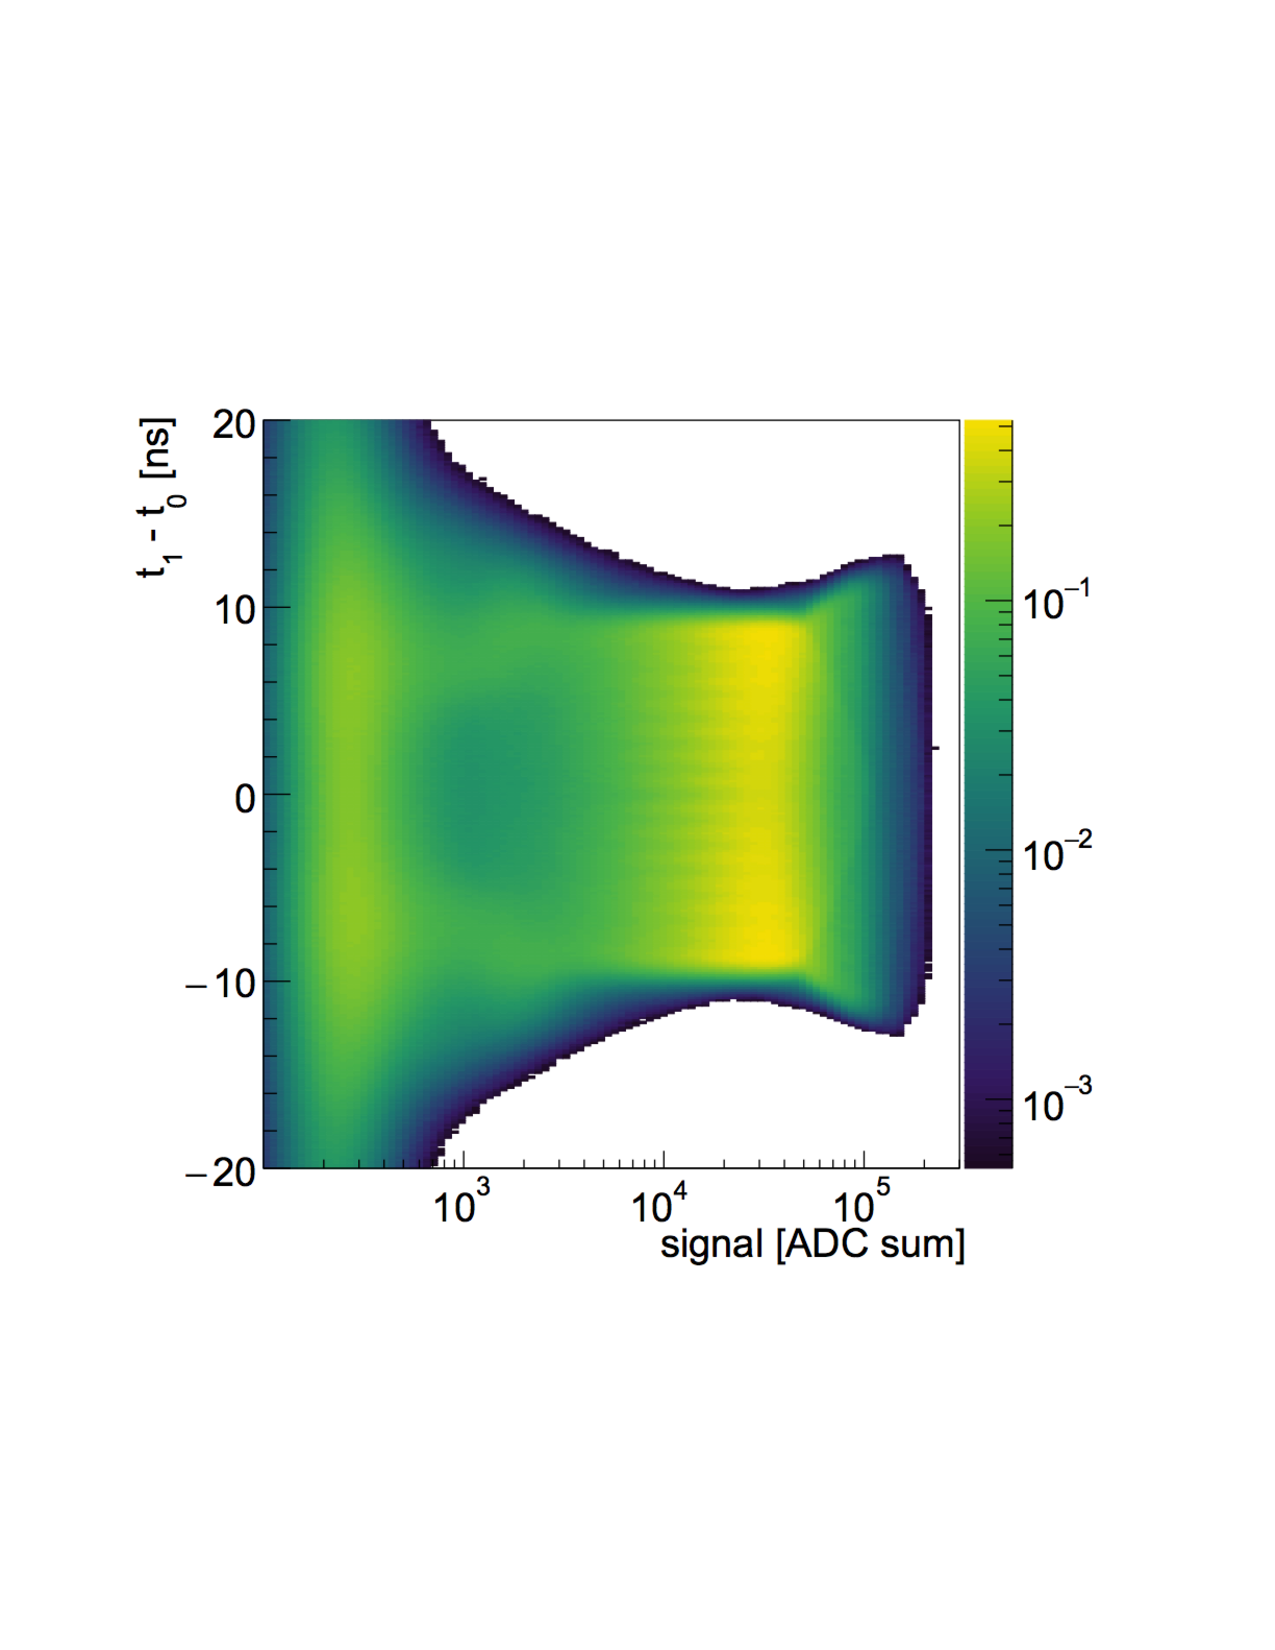
\includegraphics[width=0.95\linewidth]{tex/5-analysis-images/dt_S_Hobbes}
		\caption[Muon $dt$ versus signal amplitude]{$dt$ versus signal amplitude for through-going cosmogenic muons \cite{MM:2314}. Striping is visible at time intervals corresponding to pinwheel placement.}
		\label{fig:dtshobbes}
	\end{minipage}
	\begin{minipage}[t]{0.5\linewidth}
		\centering
		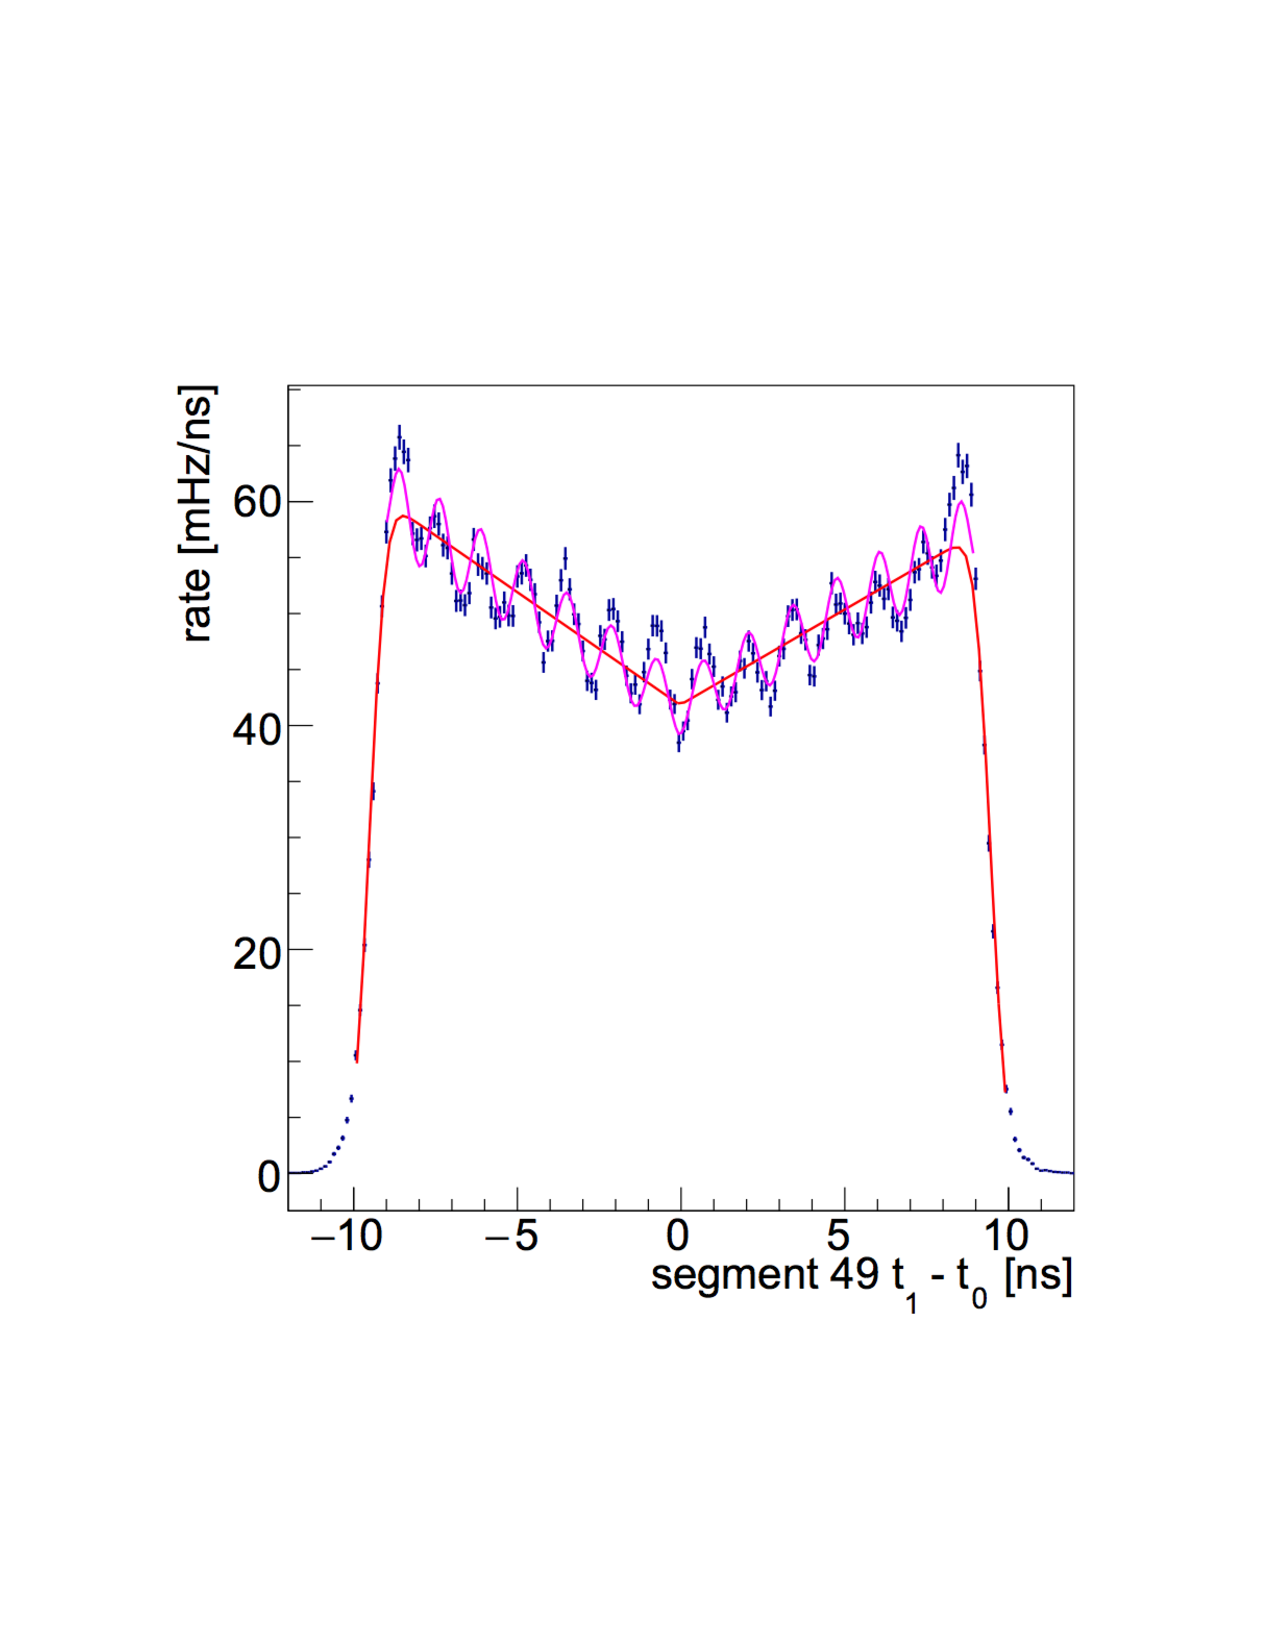
\includegraphics[width=0.85\linewidth]{tex/5-analysis-images/HobbesFit}
		\caption[Muon $dt$ for a single segment]{$dt$ of through-going muons in a single segment for events with signal amplitudes in the range  1$e$4 -  2$e$4 ADC \cite{MM:2314}. Data (blue points) are fit with an ``M"-shaped curve (red) and a sinusoidal curve (magenta).}
		\label{fig:hobbesfit}
	\end{minipage}
\end{figure}

\begin{figure}[H]
	\centering
	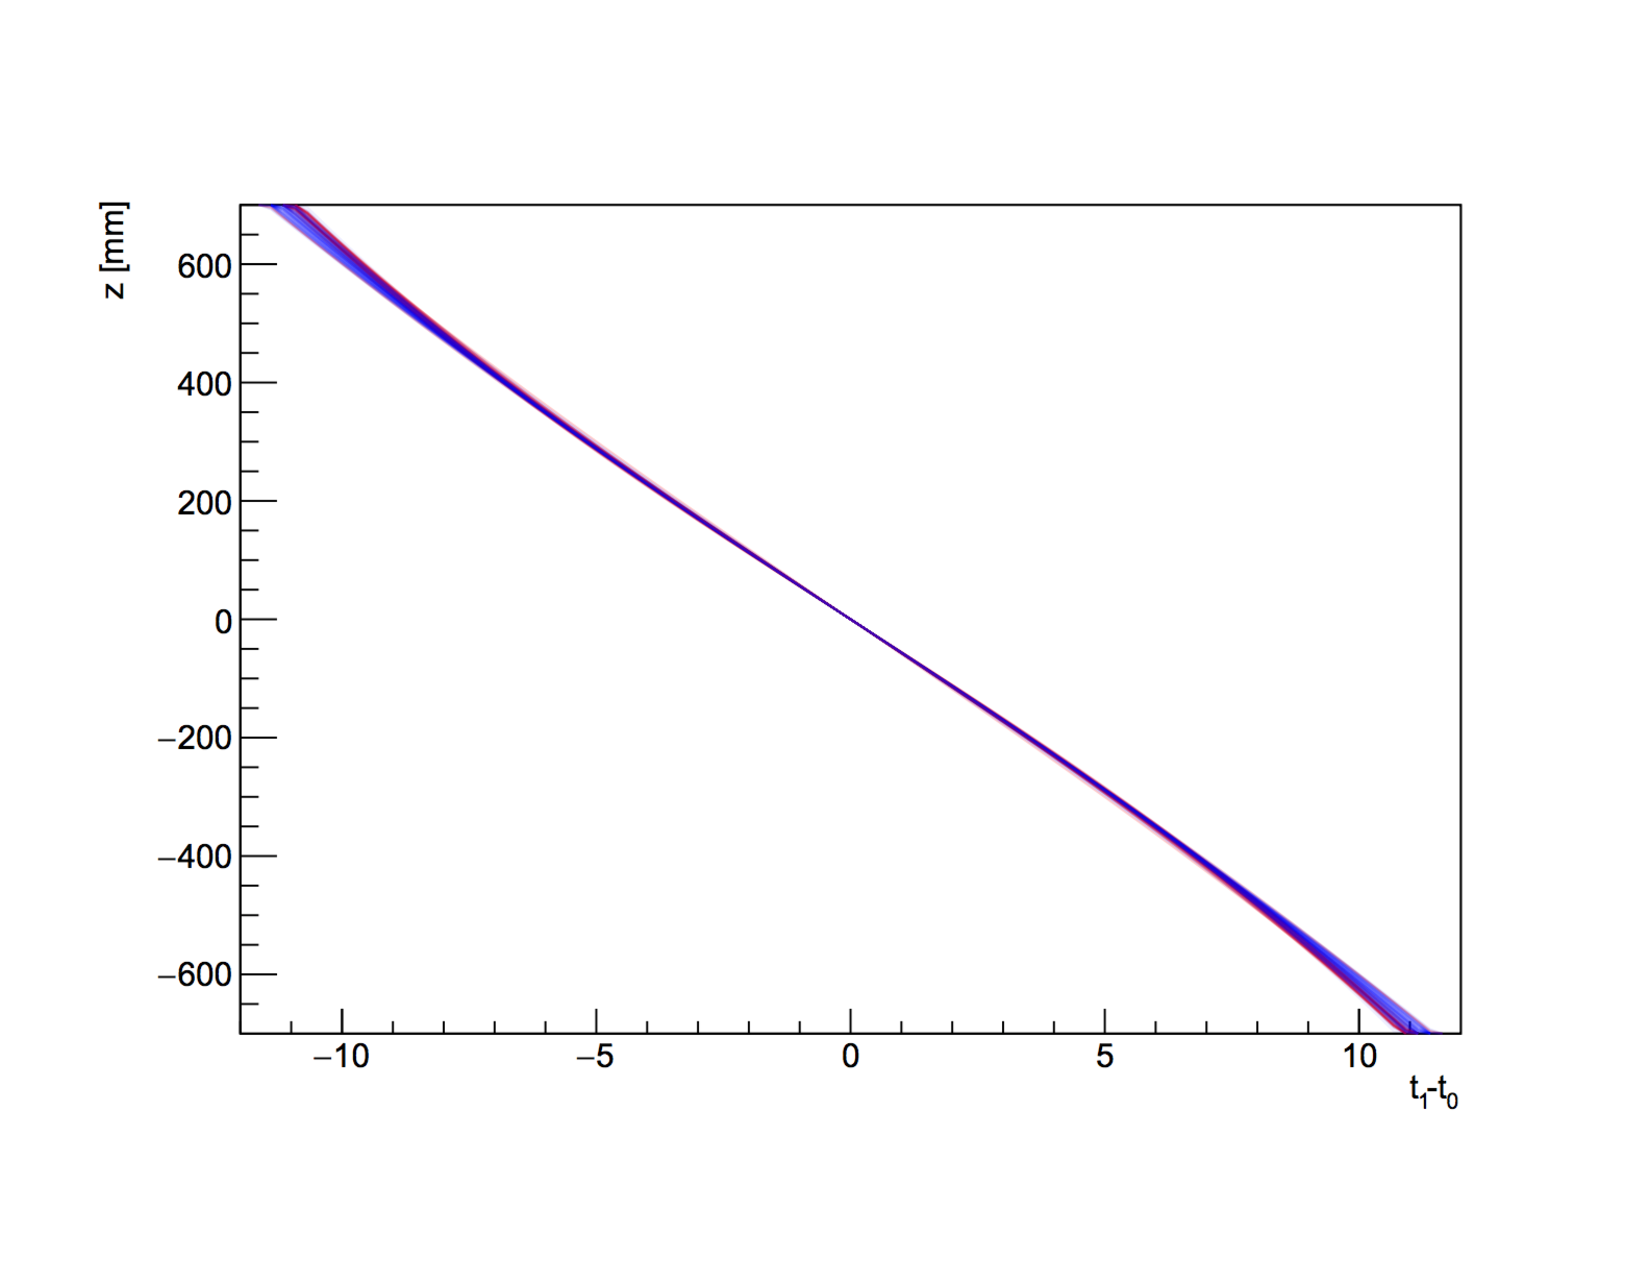
\includegraphics[width=0.5\linewidth]{tex/5-analysis-images/z_vs_dt}
	\caption[$z(dt)$ curves for all cells]{$z(dt)$ curves for all cells, extracted from fitting muon dt distributions \cite{MM:2314}. Blue: Hamamatsu segments, red: ET segments.}
	\label{fig:zvsdt}
\end{figure}

\subsection{Energy Calibration}

The energy of an event is first defined as the sum of the integral of the waveforms from both segment PMTs in ADC units. 
The next step involves converting to energy units of MeV and correcting for longitudinal light collection variation.
These procedures are performing using neutron captures on $^6$Li (nLi) because they are well understood and always peak at a quenched energy of around 0.53 MeV electron equivalent (MeVee). 

After combining the waveforms for all events, the neutron captures at the center of the segment are calibrated to 0.526 MeVee, defining the energy scale for all segments and all classes of events. 
Constraining the energy scale in this way creates a quadratic dependence of energy on position, as seen in the left panel of Figure~\ref{fig:ecorrection}.
This is corrected for by calibrating a gain factor for each PMT using two metrics. 
The first is the neutron capture signal at cell center, $S = \sqrt{S_0S_1}$, which is found by fitting the distribution in the left panel of Figure~\ref{fig:ecorrection} with a quadratic polynomial.
The second is the light ratio, $R = S_1/S_0$, at cell center which is found by fitting the distribution in the right panel of Figure~\ref{fig:ecorrection} with a cubic polynomial.
The gain factors for both PMTs are then defined as, 
\begin{equation}
	g_0 = \frac{S}{\sqrt{R}E_n} ~~~~~~~~~~~ g_1 = \frac{S\sqrt{R}}{E_n}
\end{equation}
where $E_n$ is the energy of the neutron capture peak. 


\begin{figure}[t]
	\centering
	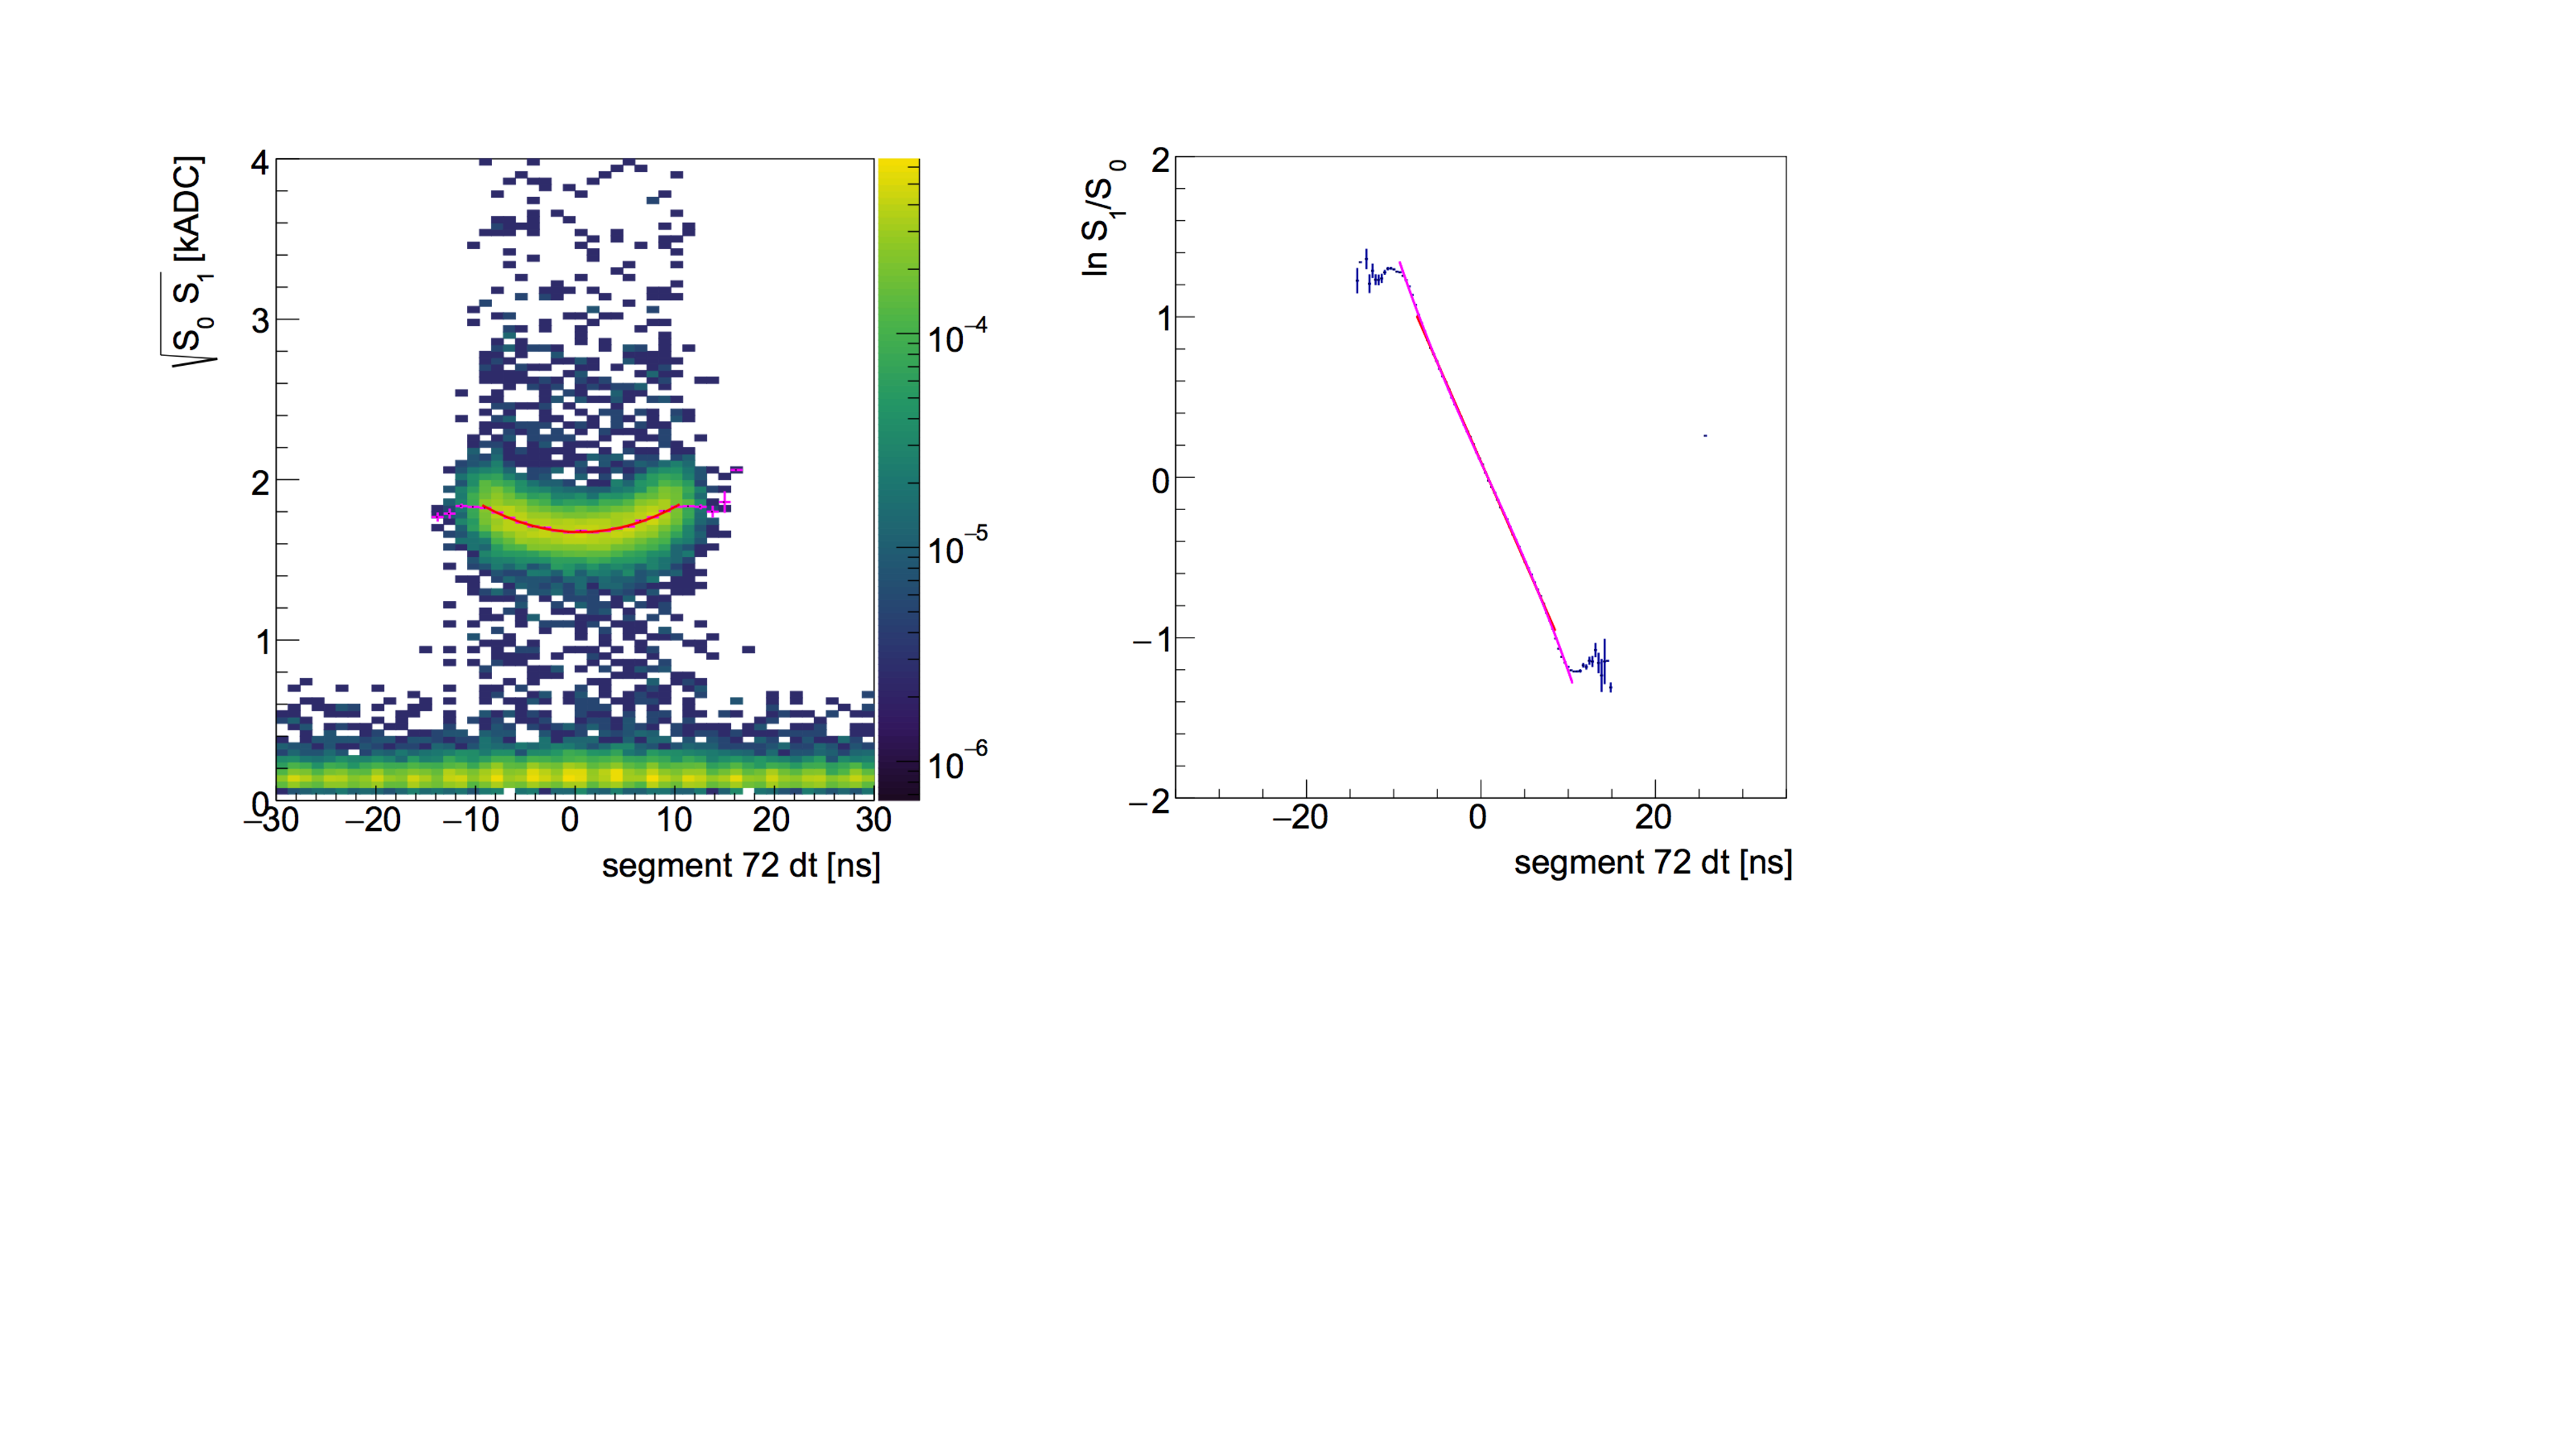
\includegraphics[width=0.9\linewidth]{tex/5-analysis-images/ECorrection}
	\caption[Energy position dependence]{(Left) Neutron capture events in one segment versus dt, with a quadratic fit in red. (Right) The ln signal ratio versus dt for muon events in one segment, with a cubic polynomial fit in magenta.}
	\label{fig:ecorrection}
\end{figure}


\section{Monte Carlo Simulation}

Due to the geometry of the PROSPECT detector and properties of the scintillator, reconstructed events are highly position and energy dependent. 
In order perform an oscillation analysis it is important to understand the detector response to incoming antineutrino events. 
This is done by modeling the detector, including all material and scintillator properties, in a GEANT-4 based simulation package hereto referred to as PROSPECT-G4 (PG4).
Monte Carlo (MC) simulations with PG4 generate a position-dependent energy response that is used to then interpret physics data. 
This can only be done if PG4 behaves the same way that the PROSPECT detector does. 
This is ensured by tuning values in PG4 to reproduce distributions measured by a variety of radioactive calibration sources and intrinsic background energy depositions.



\begin{figure}[h]
	\centering
	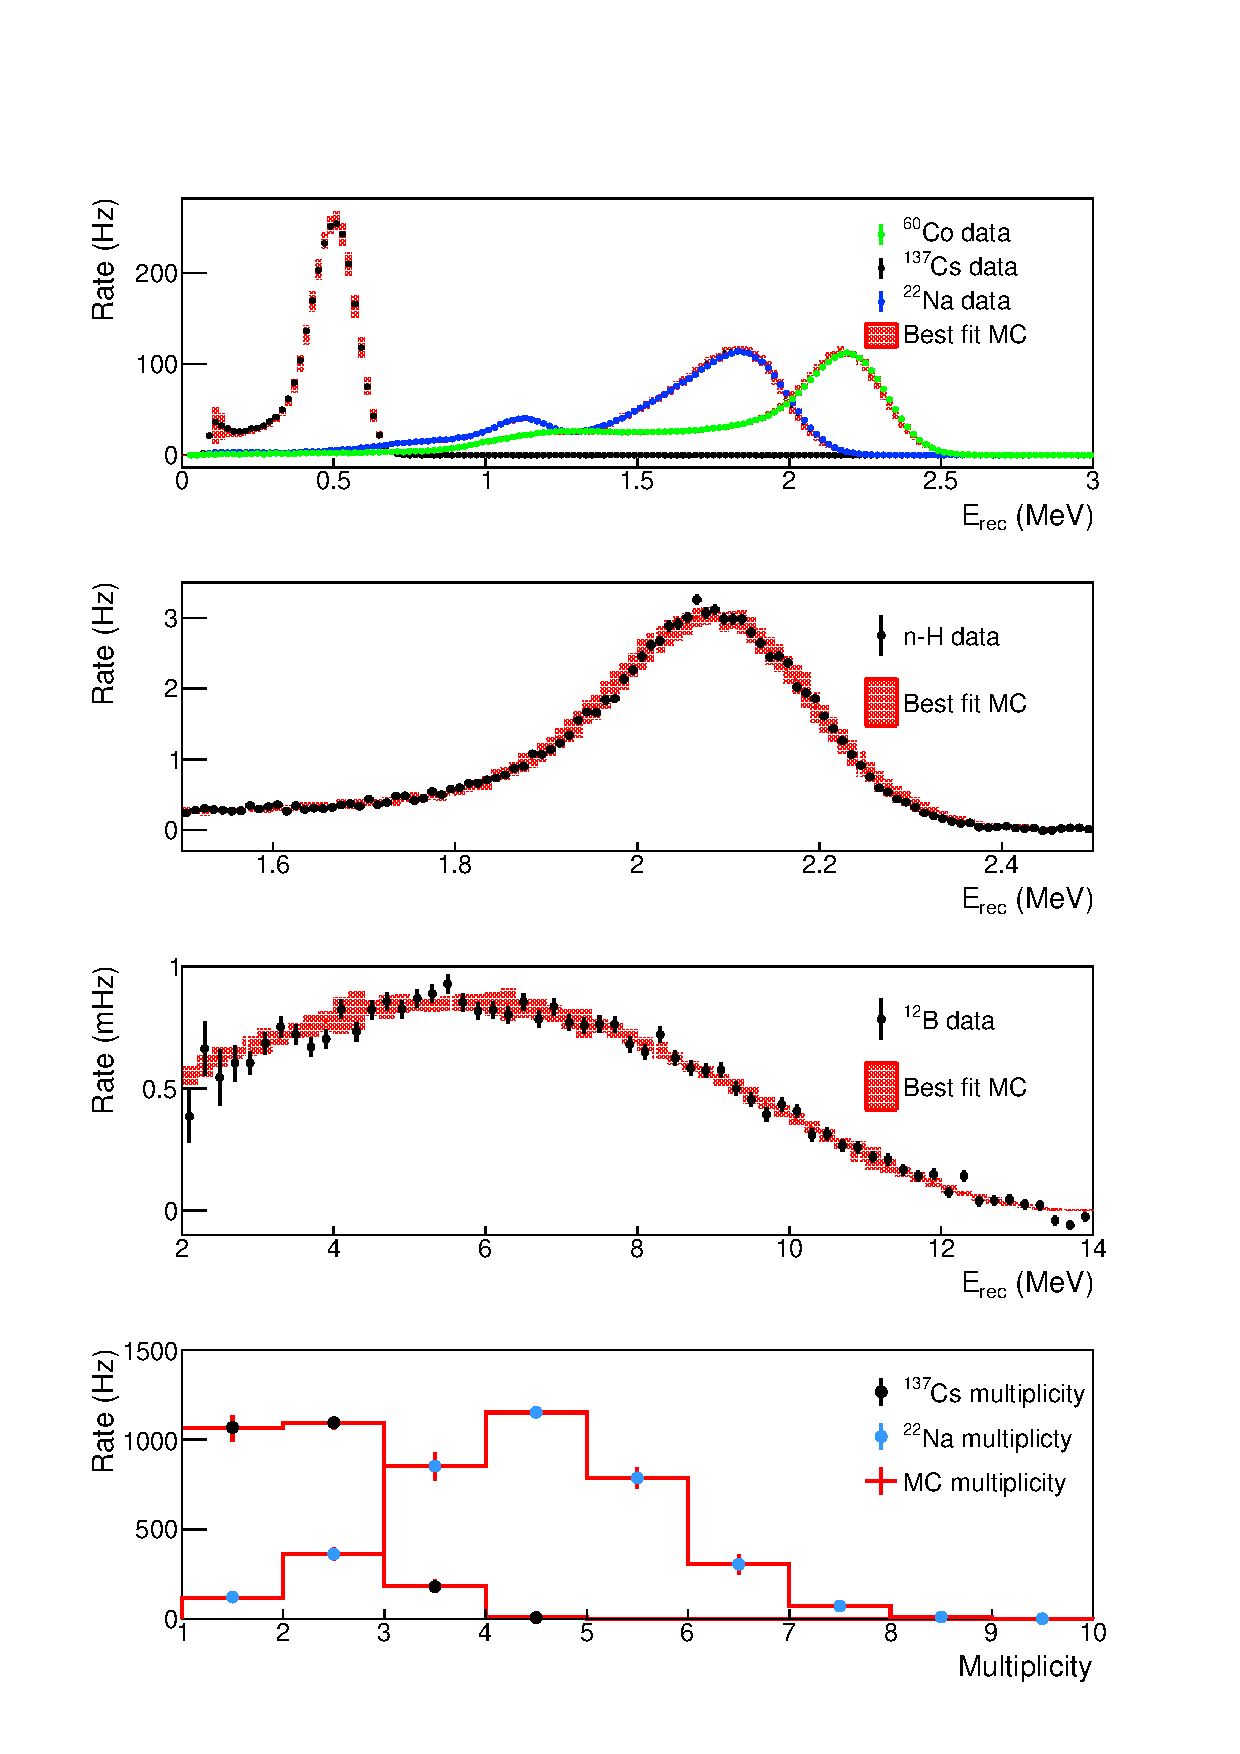
\includegraphics[width=0.7\linewidth]{tex/5-analysis-images/GammaE}
	\caption[]{Reconstructed distributions for calibration and best-fit PG4 Monte Carlo datasets \cite{XZhang:2815}. Top: $E_{rec}$ for detector-center $\gamma$-ray source deployments; Center top: $E_{rec}$ for n-H captures from a detector-center $^{252}$Cf source deployment; Center bottom: $E_{rec}$ for cosmogenically produced $^{12}$B; Bottom: pulse multiplicity for detector-center $^{137}$Cs and $^{22}$Na source deployments. Error bands indicate statistical (data) and systematic (PG4) uncertainties.}
	\label{fig:gammae}
\end{figure}

\begin{figure}[h]
	\centering
	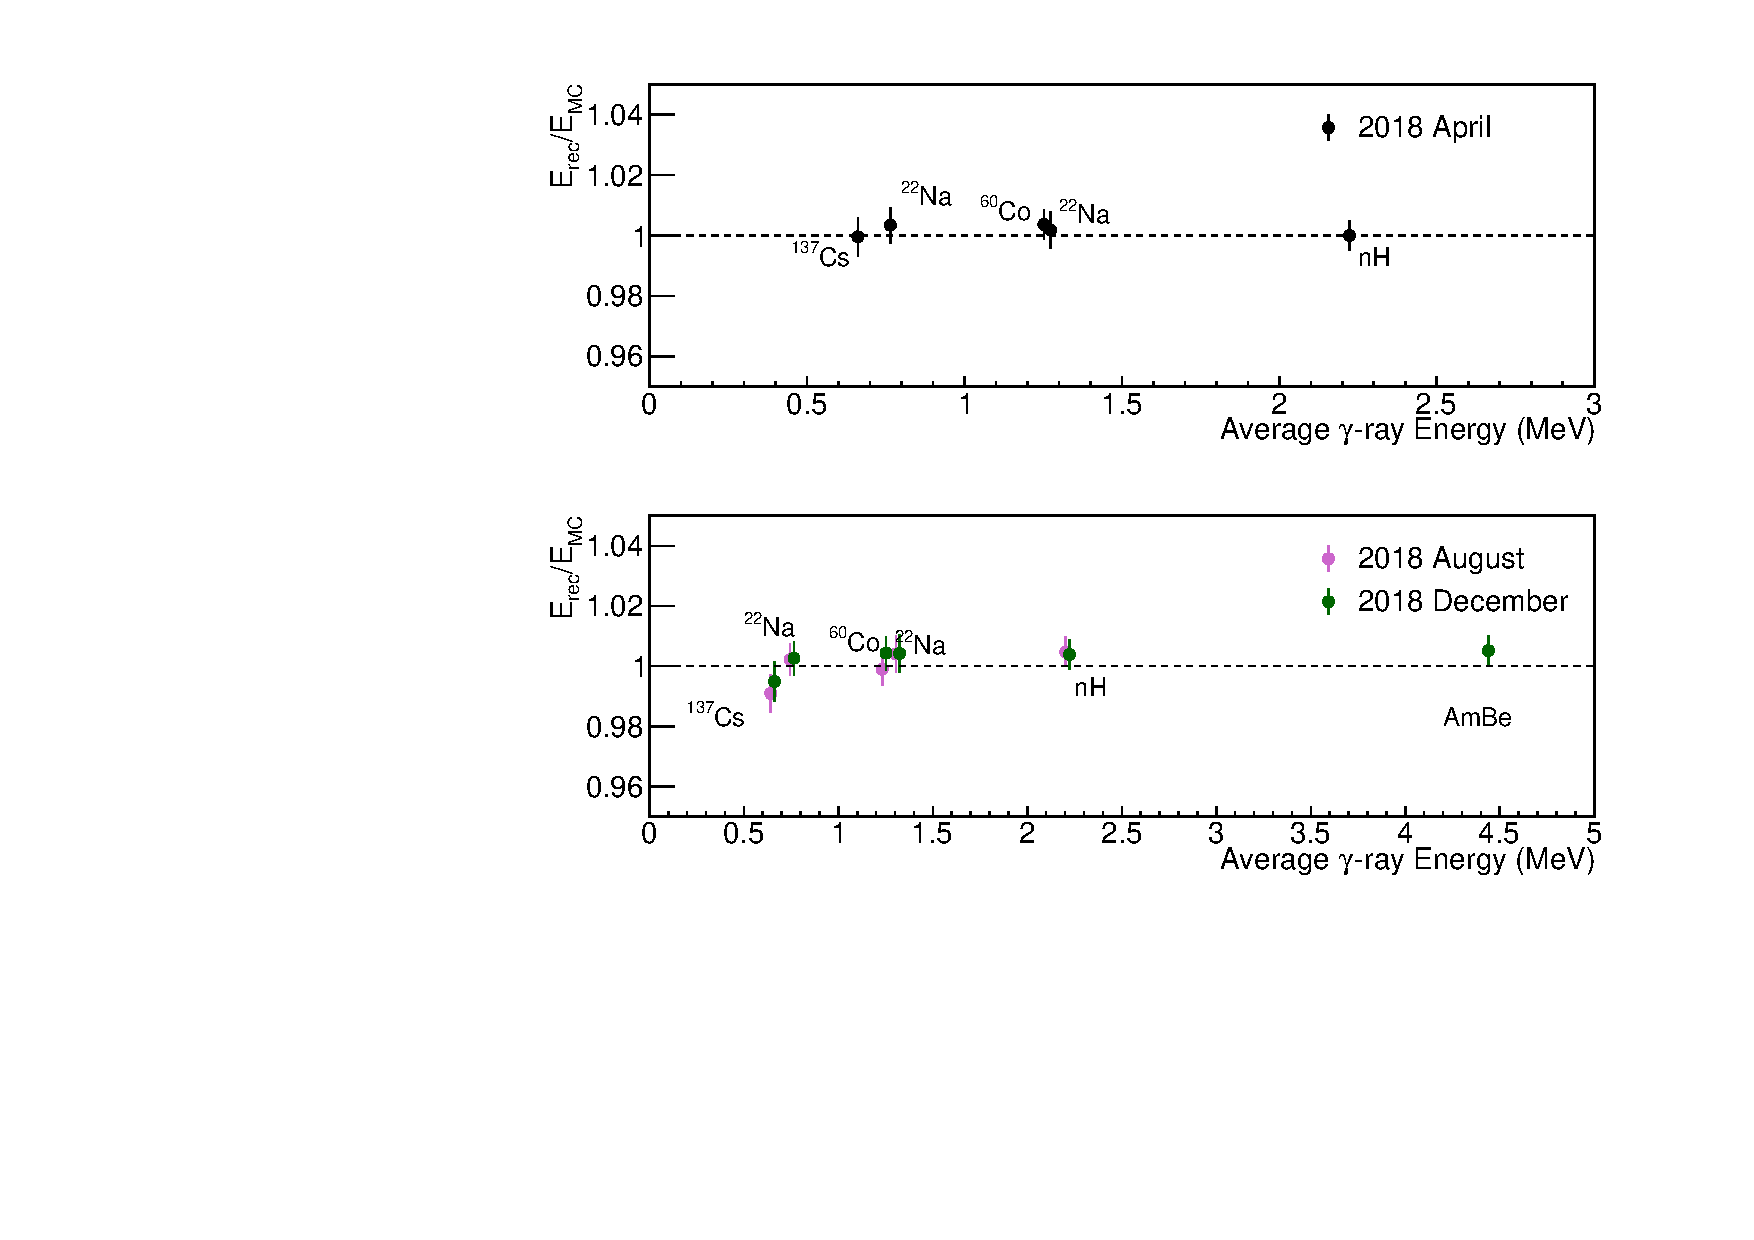
\includegraphics[width=0.7\linewidth]{tex/5-analysis-images/GammaScale}
	\caption[]{Ratios of $\gamma$ calibration source reconstructed energy peak locations between data and PG4 Monte Carlo simulations utilizing best-fit energy response modeling, plotted versus mean true gamma energy \cite{XZhang:2815}. Error bands indicate statistical and systematic uncertainties. Top: ratios for calibration source datasets used in the determination of the best-fit PG4 response model. Bottom: ratios for calibration source datasets taken during different run periods. Ratios for all datasets are within $\sim$1\% of unity, indicating excellent response modeling in PG4 for a wide variety of signal energies and multiplicities.}
	\label{fig:gammascale}
\end{figure}

\begin{figure}[h]
	\centering
	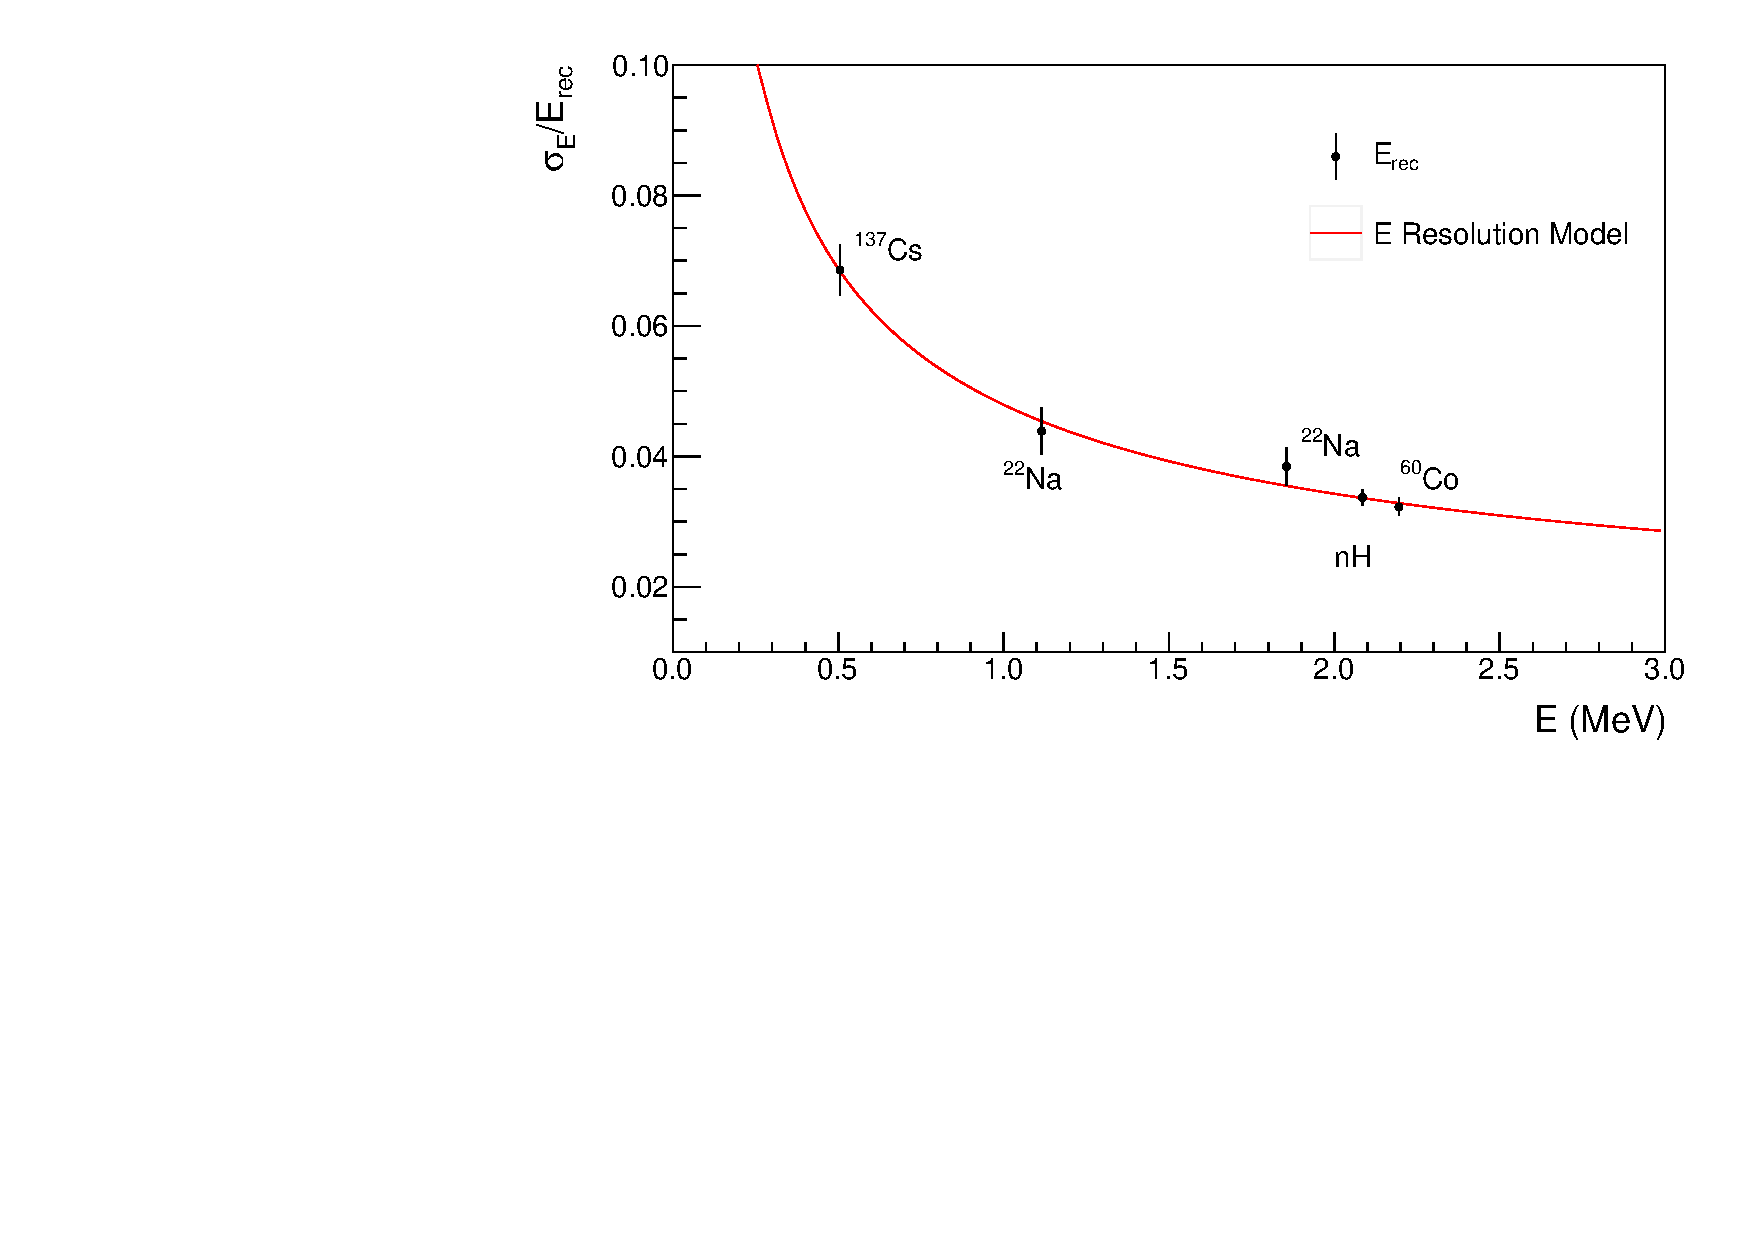
\includegraphics[width=0.7\linewidth]{tex/5-analysis-images/GammaRes}
	\caption[]{Fractional PG4-modeled energy resolution variation versus mean true gamma energy \cite{XZhang:2815}. Error bands indicate statistical and systematic uncertainties. Good agreement is visible between the PG4 model and the pictured gamma calibration datasets.}
	\label{fig:gammares}
\end{figure}



